\include{Preamble}

\title{Signed Distance Fields}
\subtitle{A Modern Approach to Shape Representation in Graphics}
\author{Md. Miraj Hasan (2005084)\\
Wahid Al Azad Navid (2005089)}
\institute{Department of Computer Science and Engineering\\Bangladesh University of Engineering and Technology (BUET)}

\begin{document}

\begin{frame}
  \titlepage
\end{frame}

\begin{frame}{Index}
  \vspace{0.5cm}
  \tiny
  \tableofcontents
\end{frame}

\section{Introduction}
\begin{frame}{What are Signed Distance Fields?}
  \begin{conceptbox}{Definition}
    A \textbf{Signed Distance Field (SDF)} is a function that gives the shortest distance between any point and the surface of a shape.
    \\~\\
    \pause % First pause: show only the definition above
    The sign indicates:
    \begin{itemize}
      \item<2-> Negative: \textit{inside} the shape
      \item<3-> Positive: \textit{outside} the shape
      \item<4-> Zero: \textit{on the surface}
    \end{itemize}
  \end{conceptbox}
\end{frame}

\section{Mathematical Foundation}
\begin{frame}{Mathematical Definition of SDF}
  \begin{mathbox}{Formal Expression}
    \[
      f(\mathbf{x}) = \pm \min_{\mathbf{p} \in \partial \Omega} \|\mathbf{x} - \mathbf{p}\|
    \]
    \pause
    \begin{itemize}[<+->]
      \item $\mathbf{x}$ = arbitrary point
      \item $\partial \Omega$ = surface boundary
      \item $f(\mathbf{x}) < 0$ if inside, $> 0$ if outside
    \end{itemize}
  \end{mathbox}
\end{frame}


\section{Applications}
\begin{frame}{Where are SDFs Used?}
  \begin{itemize}
    \item Real-time rendering and raymarching
    \item Font rendering and anti-aliasing
    \item Collision detection and physics
    \item Procedural modeling and morphing
    \item Implicit surfaces and shape blending
  \end{itemize}
\end{frame}

\section{Basic Shapes as SDFs}
\begin{frame}{SDFs for Primitive Shapes}
  \begin{itemize}
    \item \textbf{Sphere:} $f(\mathbf{x}) = \|\mathbf{x} - \mathbf{c}\| - r$
    \item \textbf{Box:} Uses component-wise signed distance
    \item \textbf{Plane, Torus, etc.}: Custom distance functions
  \end{itemize}
  \begin{conceptbox}{Key Benefit}
    Complex shapes can be formed using simple operations like union, intersection, and subtraction.
  \end{conceptbox}
\end{frame}

\section{SDF Raymarching}
\begin{frame}{Raymarching with SDFs}
  \begin{conceptbox}{Algorithm}
    \begin{enumerate}
      \item<1-> Cast a ray from the eye
      \item<2-> At each step, query the SDF to get the distance to the closest object
      \item<3-> Advance along the ray by that distance
      \item<4-> Stop when distance $< \varepsilon$ (or max steps)
    \end{enumerate}
  \end{conceptbox}
\end{frame}

\begin{frame}{Raymarching with Multiple Objects}
  \centering
  \vspace{0.5cm}
  % No \only<5-> here. Let the picture’s own <1->, <2->… drive the animation.
  \resizebox{0.8\linewidth}{!}{% raymarching_diagram.tex  (NO \begin{frame} ... \end{frame} here)
\begin{tikzpicture}[scale=1]
  % Camera
  \node[eye] (eye) at (0,0) {\faIcon{eye}};

  % Ray path
  \draw[ray] (eye) -- (7,0);

  % --- Objects (two SDF shapes) ---
  \node[sphere, fill=ObjectColor!35, minimum size=1.0cm] at (3.6,1.0) {};
  \node[above right] at (4.1,0.6) {\tiny \objectcolor{Object A}};

  \node[sphere, fill=ObjectColor!40, minimum size=2.0cm] at (6.5,0.0) {};
  \node[below] at (6.5,-1.0) {\footnotesize \objectcolor{Object B}};

  % --- March steps (appear one by one) ---
  \onslide<1->{\draw[AccentColor, thick, dashed] (1.6,0) circle (1.6);}  % r1
  \onslide<2->{\draw[AccentColor, thick, dashed] (3.2,0) circle (0.25);}  % r2
  \onslide<3->{\draw[AccentColor, thick, dashed] (3.45,0) circle (0.18);} % r3
  \onslide<4->{\draw[AccentColor, thick, dashed] (3.63,0) circle (0.12);} % r4
  \onslide<5->{\draw[AccentColor, thick, dashed] (3.75,0) circle (0.90);} % r5
  \onslide<6->{\draw[AccentColor, thick, dashed] (4.65,0) circle (0.60);} % r6
  \onslide<7->{\draw[AccentColor, thick, dashed] (5.25,0) circle (0.30);} % r7

\end{tikzpicture}
}
\end{frame}





\section{Font Rendering}
\begin{frame}{High-Quality Fonts with SDFs}
  \begin{columns}
    \begin{column}{0.6\textwidth}
      \begin{conceptbox}{Valve's Technique}
        \begin{itemize}
          \item Glyphs stored as SDFs in textures
          \item Smooth scaling and edge rendering
          \item Great for HUDs and UIs in games
        \end{itemize}
      \end{conceptbox}
    \end{column}
    \begin{column}{0.4\textwidth}
      \centering
      \resizebox{\linewidth}{!}{
        \begin{tikzpicture}[scale=1.2]
  % Pixel grid background
  \foreach \x in {0,...,5} {
    \foreach \y in {0,...,4} {
      \pgfmathsetmacro{\val}{int(100 - abs(\x-2.5)*30 - abs(\y-2)*30)}
      \fill[gray!\val!white] (\x,-\y) rectangle ++(1,-1);
    }
  }

  % Outline of glyph "A"
  \draw[PrimaryColor, ultra thick] (1,-1) -- (2.5,-4) -- (4,-1);
  \draw[PrimaryColor, ultra thick] (1.8,-2.5) -- (3.2,-2.5);

  \node[above] at (2.5,0.5) {\small SDF Texture for Letter A};
\end{tikzpicture}

      }
    \end{column}
  \end{columns}
\end{frame}

\section{Collision Detection}
\begin{frame}{Collision Detection with SDFs}
  \begin{conceptbox}{Key Idea}
    The signed distance tells how far one object is from another. 
    If the value is negative, it means collision.
  \end{conceptbox}

  \begin{itemize}
    \item<1-> Efficient for character and object physics
    \item<2-> Simple penetration depth calculation
    \item<3-> Used in soft-body and rigid-body physics engines
  \end{itemize}

  \vspace{0.5cm}
  \centering
  \only<4->{\resizebox{0.4\linewidth}{!}{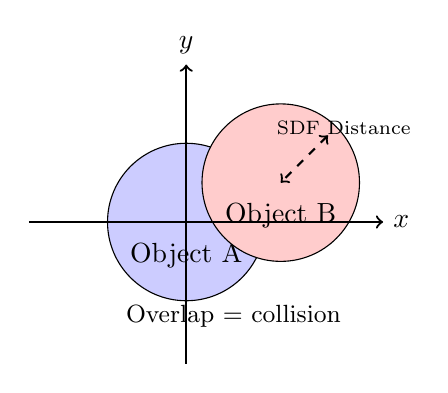
\begin{tikzpicture}
  \draw[fill=blue!20] (0,0) circle (1) node[below=4pt] {Object A};
  \draw[fill=red!20] (1.2,0.5) circle (1) node[below=4pt] {Object B};

  \draw[->, thick] (-2, 0) -- (2.5, 0) node[right] {$x$};
  \draw[->, thick] (0, -1.8) -- (0, 2) node[above] {$y$};

  \node at (0.6, -1.2) {\small Overlap = collision};
  \draw[<->, dashed, thick] (1.8,1.1) -- (1.2,0.5);
  \node at (2,1.2) {\scriptsize SDF Distance};
\end{tikzpicture}
}}
\end{frame}



\section{Procedural Modeling}
\begin{frame}{Procedural Modeling and Morphing}
  \begin{conceptbox}{Using SDF Operations}
    You can build complex models using:
    \begin{itemize}
      \item \texttt{Union}: $f = \min(f_1, f_2)$
      \item \texttt{Intersection}: $f = \max(f_1, f_2)$
      \item \texttt{Difference}: $f = \max(f_1, -f_2)$
    \end{itemize}
  \end{conceptbox}

  \vspace{0.3cm}
  \centering
  \resizebox{0.75\linewidth}{!}{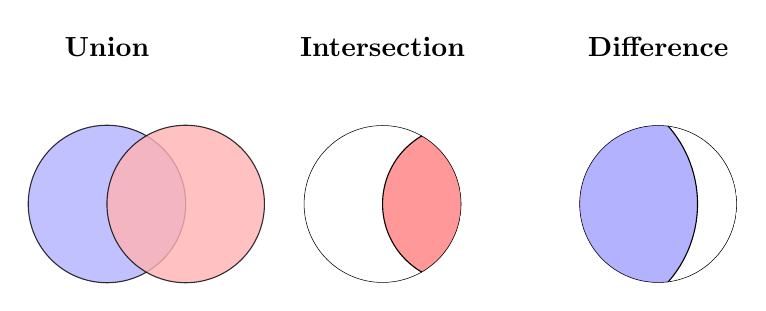
\begin{tikzpicture}
  % Labels
  \node at (-3.5,2) {\textbf{Union}};
  \node at (0,2)     {\textbf{Intersection}};
  \node at (3.5,2)   {\textbf{Difference}};

  % Union
  \begin{scope}[shift={(-3.5,0)}]
    \draw[fill=blue!30,opacity=0.8] (0,0) circle (1);
    \draw[fill=red!30,opacity=0.8] (1,0) circle (1);
  \end{scope}

  % Intersection
  \begin{scope}[shift={(0,0)}]
    \clip (0,0) circle (1);
    \fill[red!40] (1,0) circle (1);
    \draw (0,0) circle (1);
    \draw (1,0) circle (1);
  \end{scope}

  % Difference
  \begin{scope}[shift={(3.5,0)}]
    \clip (0,0) circle (1);
    \fill[blue!30] (-1,0) circle (1.5);
    \draw (0,0) circle (1);
    \draw (-1,0) circle (1.5);
  \end{scope}
\end{tikzpicture}
}
\end{frame}

\section{Shape Blending}
\begin{frame}{Implicit Surfaces and Blending}
  \begin{conceptbox}{Smooth Transitions}
    \only<1->{SDFs allow smooth blending between shapes using interpolation:}
    \only<2->{\[
      f(x) = \text{lerp}(f_1(x), f_2(x), \alpha)
    \]}
    \only<3->{or soft union: \[
      f = -\log(e^{-k f_1} + e^{-k f_2})/k
    \]}
  \end{conceptbox}

  \vspace{0.3cm}
  \centering
  \only<4->{\resizebox{0.75\linewidth}{!}{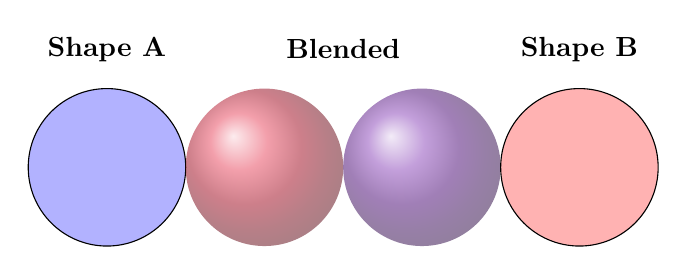
\begin{tikzpicture}
  % Left shape
  \begin{scope}[shift={(-3,0)}]
    \node at (0,1.5) {\textbf{Shape A}};
    \draw[fill=blue!30] (0,0) circle (1);
  \end{scope}

  % Right shape
  \begin{scope}[shift={(3,0)}]
    \node at (0,1.5) {\textbf{Shape B}};
    \draw[fill=red!30] (0,0) circle (1);
  \end{scope}

  % Blended shape
  \begin{scope}[shift={(0,0)}]
    \node at (0,1.5) {\textbf{Blended}};
    \shade[ball color=purple!50!red, opacity=0.5] (-1,0) circle (1);
    \shade[ball color=purple!50!blue, opacity=0.5] (1,0) circle (1);
  \end{scope}
\end{tikzpicture}
}}
\end{frame}




\section{Generating SDFs}
\begin{frame}{How are SDFs Generated?}
  \begin{itemize}
    \item \textbf{Analytical}: Direct formulas for simple shapes
    \item \textbf{Voxel-based}: Grids for complex models
    \item \textbf{From images}: Euclidean distance transform
    \item \textbf{GPU-based}: Jump Flood Algorithm (JFA)
  \end{itemize}
\end{frame}

\section{Modern Extensions}
\begin{frame}{Recent Innovations}
  \begin{itemize}
    \item \textbf{Neural SDFs}: Learnable representations (e.g., NeRF)
    \item \textbf{Volumetric rendering}: Clouds, fog, soft shadows
    \item \textbf{SDF octrees}: Efficient memory and level-of-detail
  \end{itemize}
\end{frame}

\section{Conclusion}
\begin{frame}{Conclusion}
  \begin{conceptbox}{Key Takeaways}
    \begin{itemize}
      \item Compact, efficient way to represent shapes
      \item Ideal for GPU and real-time applications
      \item Extensible to AI, physics, VFX, and more
    \end{itemize}
  \end{conceptbox}
\end{frame}

\end{document}
